
\section{Possible cobot Solutions} \label{ch:UR}

This section is taking 3 different cobots into consideration for a possible solution to the case description.

\subsection{KUKA}

The KUKA company started more than a hundred years ago. They were the first to invent point welding gripper in Germany.\\
As the years goes by the KUKA company writes history by inventing the world first industrial lightweight robot with sensors in every axis.\\
\\
KUKA and Rethink are competitors since they have the same market, hence is why this project will take both in to consideration of a possible optimization of the work-cell\cite{KukaHist}.\\


\subsubsection{KUKA LBR IIWA 7 R800}
\begin{figure}[H]
    \centering
    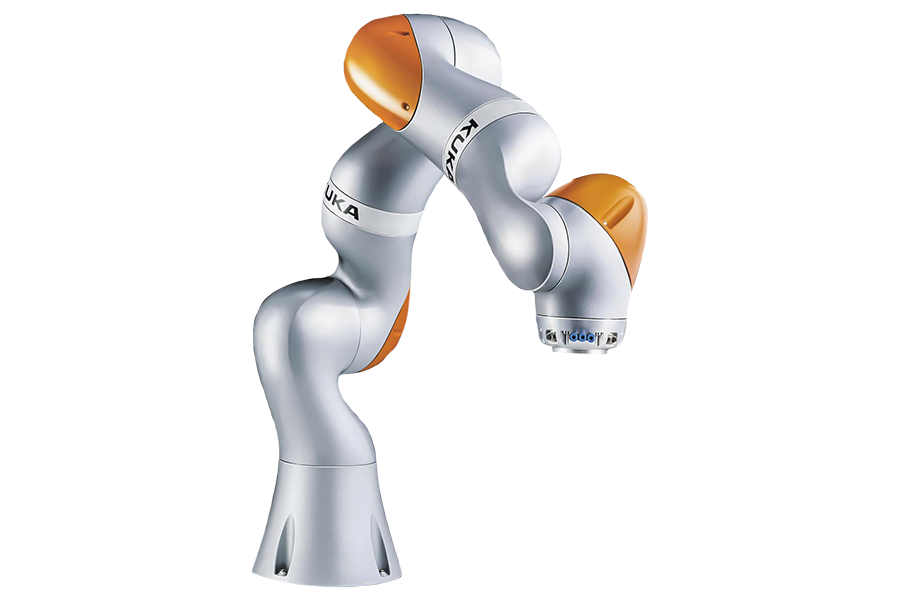
\includegraphics[width=9cm]{UR/1502895088_1.png}
    \caption{KUKA LBR IIWA 7 R800 \cite{KUKAbillede}}
    \label{fig:LBR IIWA}
\end{figure}

Here are the specification for the LBR iiwa 7 R800:\\

\begin{itemize}
    \item Weight: 23.9 kg.
    \item Payload: 7 kg.
    \item Footprint: 136 mm.
    \item Joints: Ranging from +/-120 degrees to +/-170.
    \item Operating life: 30,000 Hours.
    \item Speed: Joints = 180 degrees/sec
    \item Reach: 800-820 mm
    \item Repeatability: +/- 0.1 mm.
\end{itemize}
\cite{KukaSpec1},\cite{KukaSpec2}.

\subsection{Rethink Robotics}

Rethink robotics was founded in 2000, and are known for their invention the "Roomba Vacuum". They decided to use their knowledge of machinery in the everyday life in factories.\\
The first cobot they designed was in 2012, and was called "Baxter", see \ref{fig:Rethink},\cite{Rethink}.

\subsubsection{Baxter}
\begin{figure}[H]
    \centering
    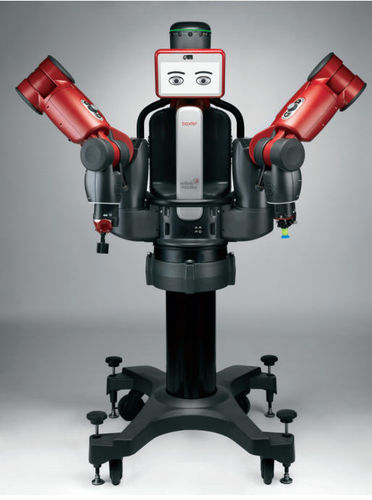
\includegraphics[width=9cm, height=9cm]{UR/baxter-robot-1.jpg}
    \caption{Baxter cobot from "Rethink Robotics"\cite{Rethinkbillede}}
    \label{fig:Rethink}
\end{figure}

\subsubsection{Specifications for Baxter}
\begin{itemize}
    \item Weight: 75 kg.
    \item Payload: 2.2 kg.
    \item Footprint: 36x32 cm.
    \item Joints: Ranging from +/-175 degrees.
    \item Operating life: Unknown.
    \item Speed: Joints = 2 to 4 sec per joint rotation.
    \item Reach: 1210 mm
    \item Repeatability: +/- 5 mm.
\end{itemize}
\cite{Rethinkspec}
\\
The Baxter robot is a highly flexible collaborative robotic manipulator, with built in sensors and cameras, that allows the robot to see and adapt to its environment.\\
The robot features embedded cameras, and force recognition, to recognize and act upon collisions. This combined with its limited force, makes the Baxter safe around humans.
The camera is 1280p x 800p with 30 frames per second, and the infrared sensor has a range of 4-40 cm. 
It also has additional sensors around the end-effector, that allows it to analyze the object it is holding. \\
One part of its flexibility is the ability to adapt to new work environments on the go, using the sensors around its head. Another part is the ability to move. The Baxter robot can be placed on a four legged pedestal, which allows it to move around. \\
While this robot could have been a good consideration for the task, its availability is limited to certain countries, and is not available in Denmark\cite{rethinkbaxter}.

\subsection{UR}

Universal Robots was founded in 2005 by a group of Danish engineers. Their thought was, that every industrial robot on the market was designed to be big, heavy and expensive. Therefore the group decided to make a smaller and more agile kind of industrial robot.\cite{Urhist}\\
Here are the specification for the UR5:\\ 

\subsubsection{Specifications for UR5}

\begin{itemize}
    \item Weight: 18.4 kg.
    \item Payload: 5 kg.
    \item Footprint: 149 mm.
    \item Joints: +/-360 degrees on all the joints.
    \item Operating life: 35,000 Hours.
    \item Speed: joints = 180 degrees/sec, tool = 1 m/sec.
    \item Reach: 850 mm.
    \item Repeatability: +/- 0.1 mm.
\end{itemize}

The materials used on all the cobots are aluminum and plastic\cite{Ur5_about}\cite{UR5_tech}.\\

\begin{figure}
    \centering
    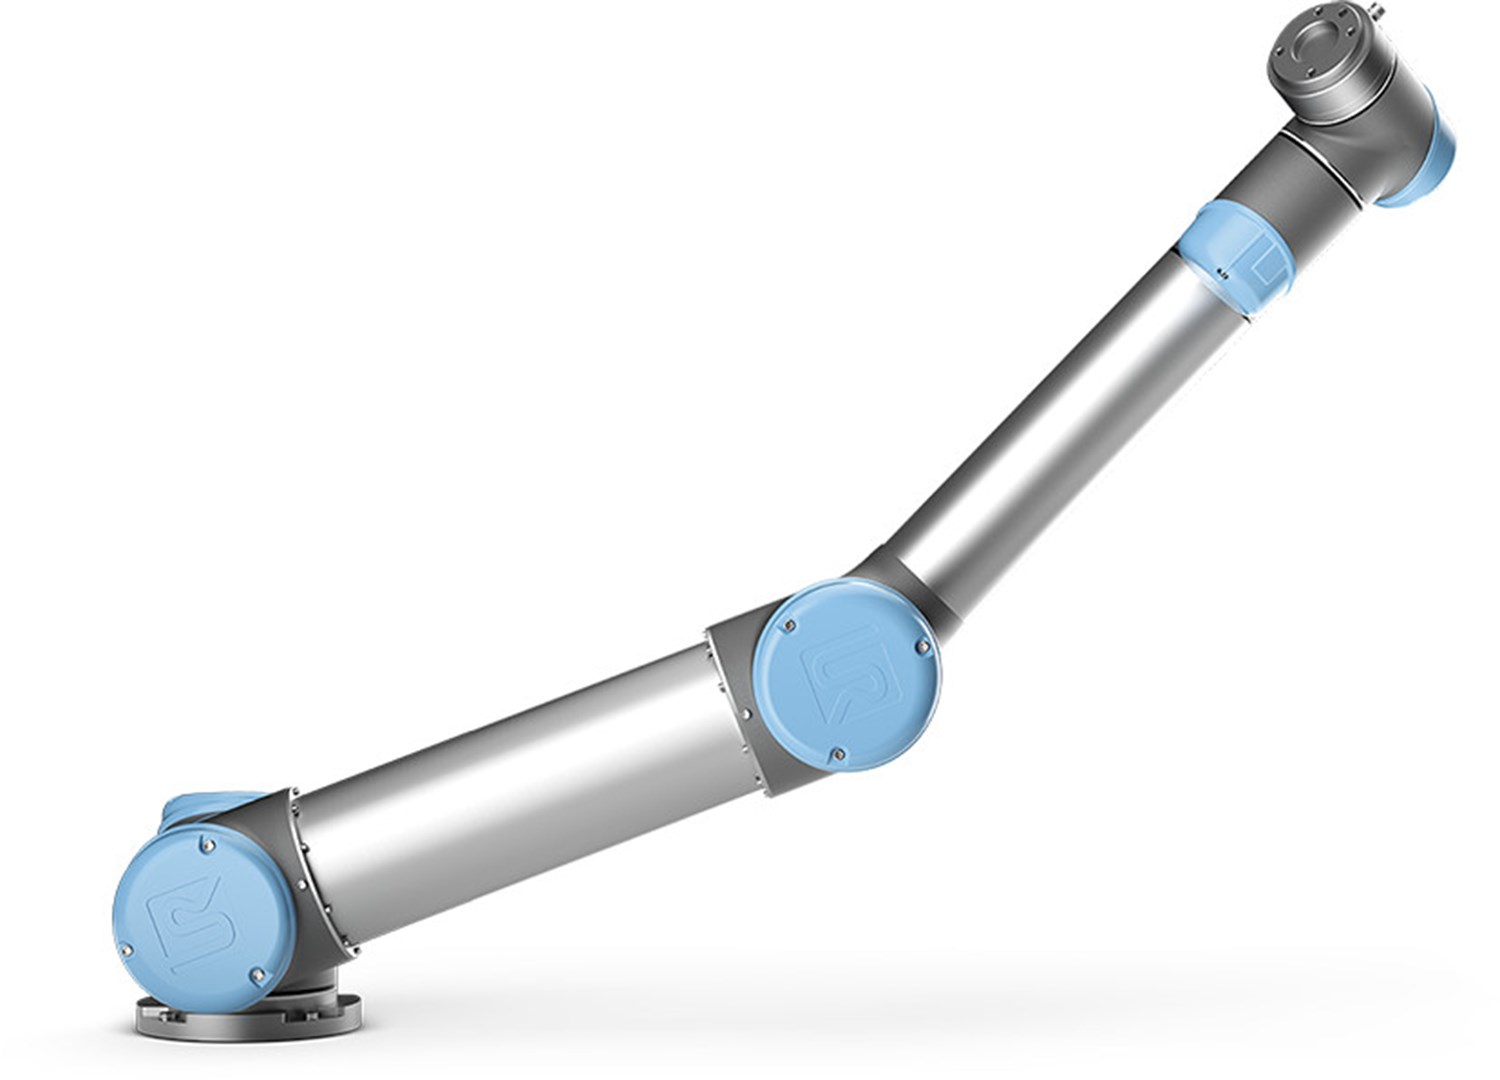
\includegraphics[width=9cm]{UR/UR5pic.jpg}
    \caption{Universal Robots UR5 \cite{UR5billede}}
    \label{fig:UR5}
\end{figure}


\subsection{Why cobots?}\label{ch:Whycobot}
Why is there a need for a cobot? A thing that is mentioned in an article about cobots, in an assembly line, is that cobots can help reduce the ergonomics stress level of the employees\cite{Coboau}. Another way this can help the production flow, is that the robot can preform some tedious task while the employee can take care of the complex tasks in the work area.\\



\subsection{Mobile platform}
A way to overcome the reach problem in the previous mentioned, could be a mobile platform where the manipulator will be placed on, so that the manipulator can be moved to reach any of the machines that the rotor has to go through to complete the work process. Usually having a mobile platform requires sensors which can give the platform a vision to move around within the work-cell\cite{doi:10.1177/1729881417718588}, furthermore it usually would require that the platform is programmed by an expert, but in this article \cite{doi:10.1177/1729881417718588} they focus on making a more user friendly platform, so that the worker at the station can program and incorporate, the mobile platform to fit into a new work situation.\\

\subsection{A rail} 
A rail could also be another solution to extend the reach of the manipulator, by installing the manipulator on or under a rail so the manipulator can move back and fourth on a single axis or in a plane like a gantry crane. This solution will require two rails where one has to be installed on top of the other on a perpendicular axis\cite{FRUNS}.

\section{End-effector}

In this section the 3 most used gripper types being used in the industry, will be explained.

\subsection{Mechanical gripper}
The End-effector which is available for the group in this project is a pneumatic driven gripper. The gripper weighs 0.5 Kg (excluding gripper fingers). It has an operation pressure range from 3 to 7 Bar and the gripper claws are operated independently\cite{MWC}.The gripper in its neutral state is open, when air pressure is applied to the gripper it will close.\\
To control the gripper, solenoid actuated valves are used. To operate the valve a voltage is applied to the solenoid and the valve will move to an open position and let air flow towards the gripper.\\
The group can use the gripper by connecting the valve to the control box of the manipulator, then use the valve through the teach pendant.\\ 

\begin{figure}[H]
    \centering
    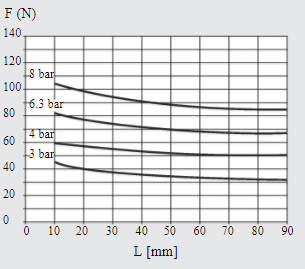
\includegraphics{TechnicalAnlysis/MWforcedia.PNG}
    \caption{This diagram shows the force object depending on the pressure and length of gripper fingers\cite{MWC}}
    \label{fig:Mvforce}
\end{figure}

\subsection{Suction / vacuum cup}
This kind of gripper is mostly used for pick and placement of non-ferrous materials, where only one surface is available to handle the material.\\ 
It functions by causing a vacuum inside the cups to hold onto.\\
This type of gripper is good for picking up objects, which are smooth, flat, and clean, and are less suitable for picking up objects with holes in it \cite{Gripper1}.\\

\subsection{Magnet gripper}
The magnetized end-effector is functioning much like the vacuum cups, where it only can hold on to a single surface on ferrous materials, instead of functioning by vacuum, it is using magnets to hold onto materials. The gripper is switching been on/off mode by pushing compressed air into the case, to push the magnet on or off see fig \cite{MagnetCite}.\\
This type of end-effector has the drawback that, if fast movements occur, there is a chance for the material to slip off its grip, this can also occur for the vacuum gripper\cite{Gripper2}.\\

\begin{figure}[H]
    \centering
    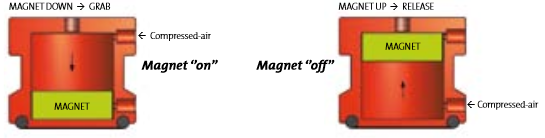
\includegraphics{TechnicalAnlysis/MagnetGripper.PNG}
    \caption{This figure shows how a basic Magnetic Gripper is turned on/off \cite{MagnetCite}}
    \label{fig:MagnetGrip}
\end{figure}

\subsection{Inflatable Gripper}
Inflatable bladder type grippers, functions like a balloon, which will be expanded once it is in the holding grip of the material, and is used to move items which requires fragile handling \cite{Gripper3}.\\

\section{Repeatability and accuracy}
When talking about Repeatability, it should not be confused with accuracy, though they are somewhat similar.\\
Repeatability is the factor of how high the spread rate is, which means a higher repeatability will cause the end-effector to reach closer to the same point on every repeat action.\\
Accuracy is the factor which tells us, how close the end-effector can be expected to reach the given position set by the user. This means a higher accuracy will lead to a diminished spread, compared to the position given in a space\cite{RepeatWhat}.\\

\begin{figure}[H]
    \centering
    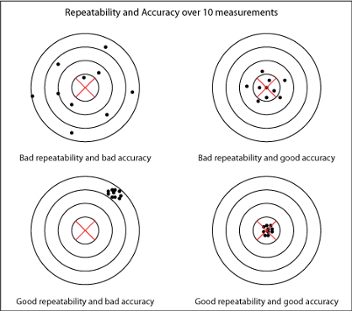
\includegraphics[width=.9\textwidth]{TechnicalAnlysis/RepeatTest.jpg}
    \caption{The difference between high/low repeatability and accuracy\cite{RepeatWhat}}
    \label{fig:Repeatability}
\end{figure}


%\subsection{Which cobot is more suitable?}

%Having the case description in mind \ref{ch:case description}, and the fact that the process must not be more than 26 seconds, before a fully functional rotor is ready.\\
%The cobots have almost similar specifications, the only major difference is the rotations of the joints. In this case a huge maneuverability is required, hence the rotation of the joints is a factor weighed highly in this process. Beside that, the only difference would be what would suit the company the most. Since Grundfos has implemented KUKA's is because it is easier to run a production-line with the same system, and the workers know these robots.\\
%The most suitable for this project is UR5.

%\subsection{Conclusion}

%Taking all of the above into consideration, some data can be included in the ideal robot for this case.\\ 
%Having an overview of the different tasks that has to be preformed and using the tools that are given, the project can get closer to a conclusion for the robot.\\
%The project has focused on two different cobots, 1 from KUKA, and 1 from UR. They are then set up to conclude which has the better specifications. By looking at nothing else than the specifications, the most suitable for this case is the UR5.\\



